% !TeX spellcheck = fr_FR
% !TeX encoding = UTF-8
% !TeX program = xelatex

% ----------------------------
% Préambule
% ----------------------------
\documentclass[10pt,a4paper]{report}
%\usepackage[utf-8]{inputenc}
%\usepackage[T1]{fontenc}
\usepackage[french]{babel}
\usepackage{amsmath}
\usepackage{amsfonts}
\usepackage{amssymb}

\usepackage{graphicx}
\usepackage{float}
%\usepackage{caption}

\usepackage{titlesec}

\usepackage{hyperref}
\usepackage{fancyhdr}

\author{Jan Schönbächler}
\title{Moodle 2021-2022 - OC 4\textsuperscript{eme} - intro à \LaTeX}


% ----------------------------
% Début du document
% ----------------------------
\begin{document}
	
	%\maketitle
	
	\parindent=0cm
	
	\chapter{Accès à Moodle Lyca}
	
	\section*{En bref\dots}
	
	Depuis la rentrée 2021-2022, l'accès à la plateforme Moodle du Lyca se fait depuis l'ENT ou via l'identité unique. Ceci crée automatiquement un nouveau compte, vers lequel vos anciennes données seront transférées, dans un délai de 24 heures.\\
	
	
	Le lien suivant explique comment se connecter à Moodle via l'identité unique, depuis l'ENT : \href{https://support.ictvs.ch/media/attachments/2021/07/20/tutoriel\_moodle\_win-fr\_2-acces-identite-unique.pdf}{tutoriel «Comment se connecter à Moodle avec mon identité unique»}\\
	
	
	\textbf{Attention :} Le transfert vers le nouveau compte prend 24 heures. Toutes les actions effectuées durant ce laps de temps seront perdues. Il est donc recommandé de se connecter une première fois avec l'identité unique, puis de se déconnecter et de patienter 24 heures avant d’utiliser à nouveau Moodle.\\
	
	Si vous utilisez la connexion via l’application Moodle Mobile (sur votre smartphone), elle doit également être mise à jour : \href{https://support.ictvs.ch/media/attachments/2021/07/22/tutoriel\_moodle\_android-fr\_2-acces-identite-unique-mobile.pdf}{tutoriel «Comment se connecter à Moodle Mobile avec mon identité unique»}
	
	
	\section{Connexion à Moodle via l'\href{https://edu.vs.ch}{ENT}}
	
	\fancyhead[LO,R]{\bfseries 1  Connexion à Moodle via l'\href{https://edu.vs.ch}{ENT}}
	
	Première possibilité : se connecter à Moodle via l'ENT, disponible à l'adresse \href{https://edu.vs.ch}{https://edu.vs.ch}, où vous entrez votre nom d'utilisateur et mot de passe habituels (cf. figure \ref{fig:accesENT}).
	
	% TODO: \usepackage{graphicx} required
	\begin{figure}[H]
		\centering
		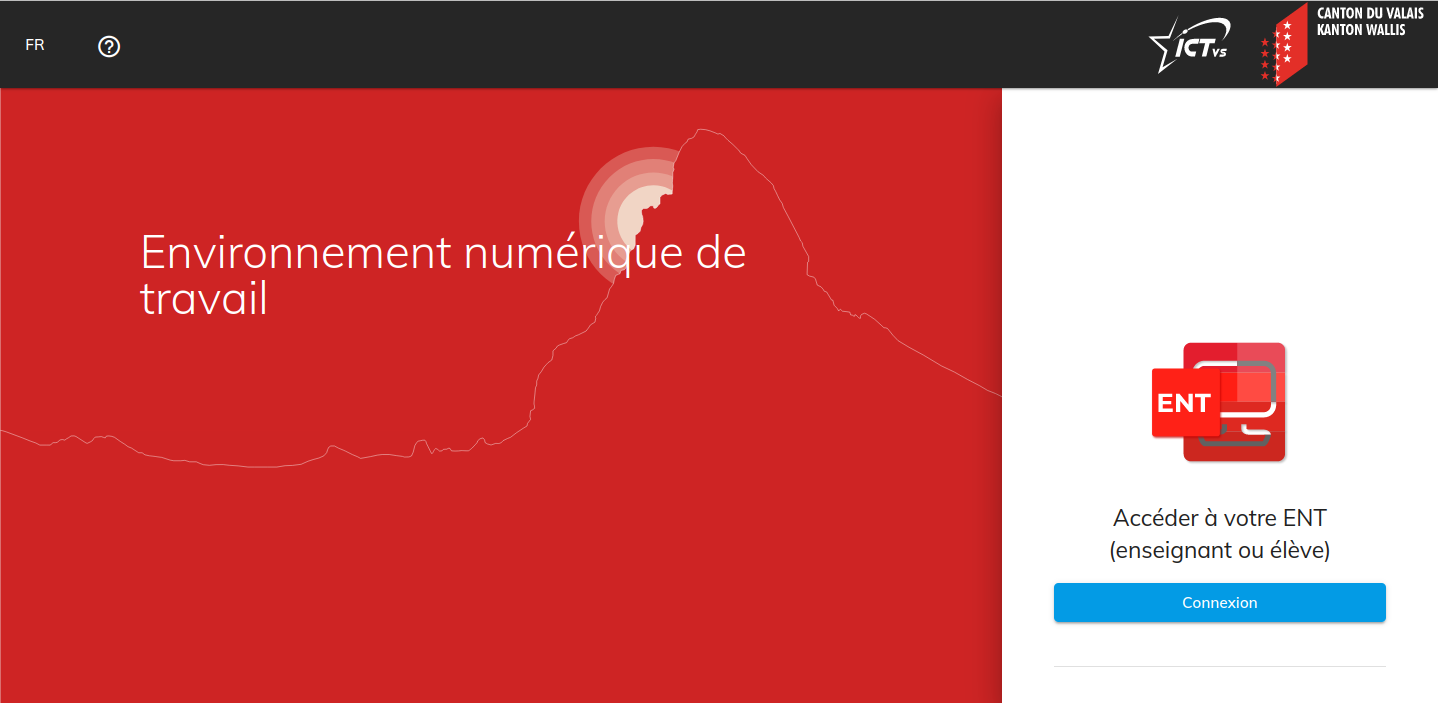
\includegraphics[width=0.8\linewidth]{images/capture_ENT_20210811}\\ [2ex]
		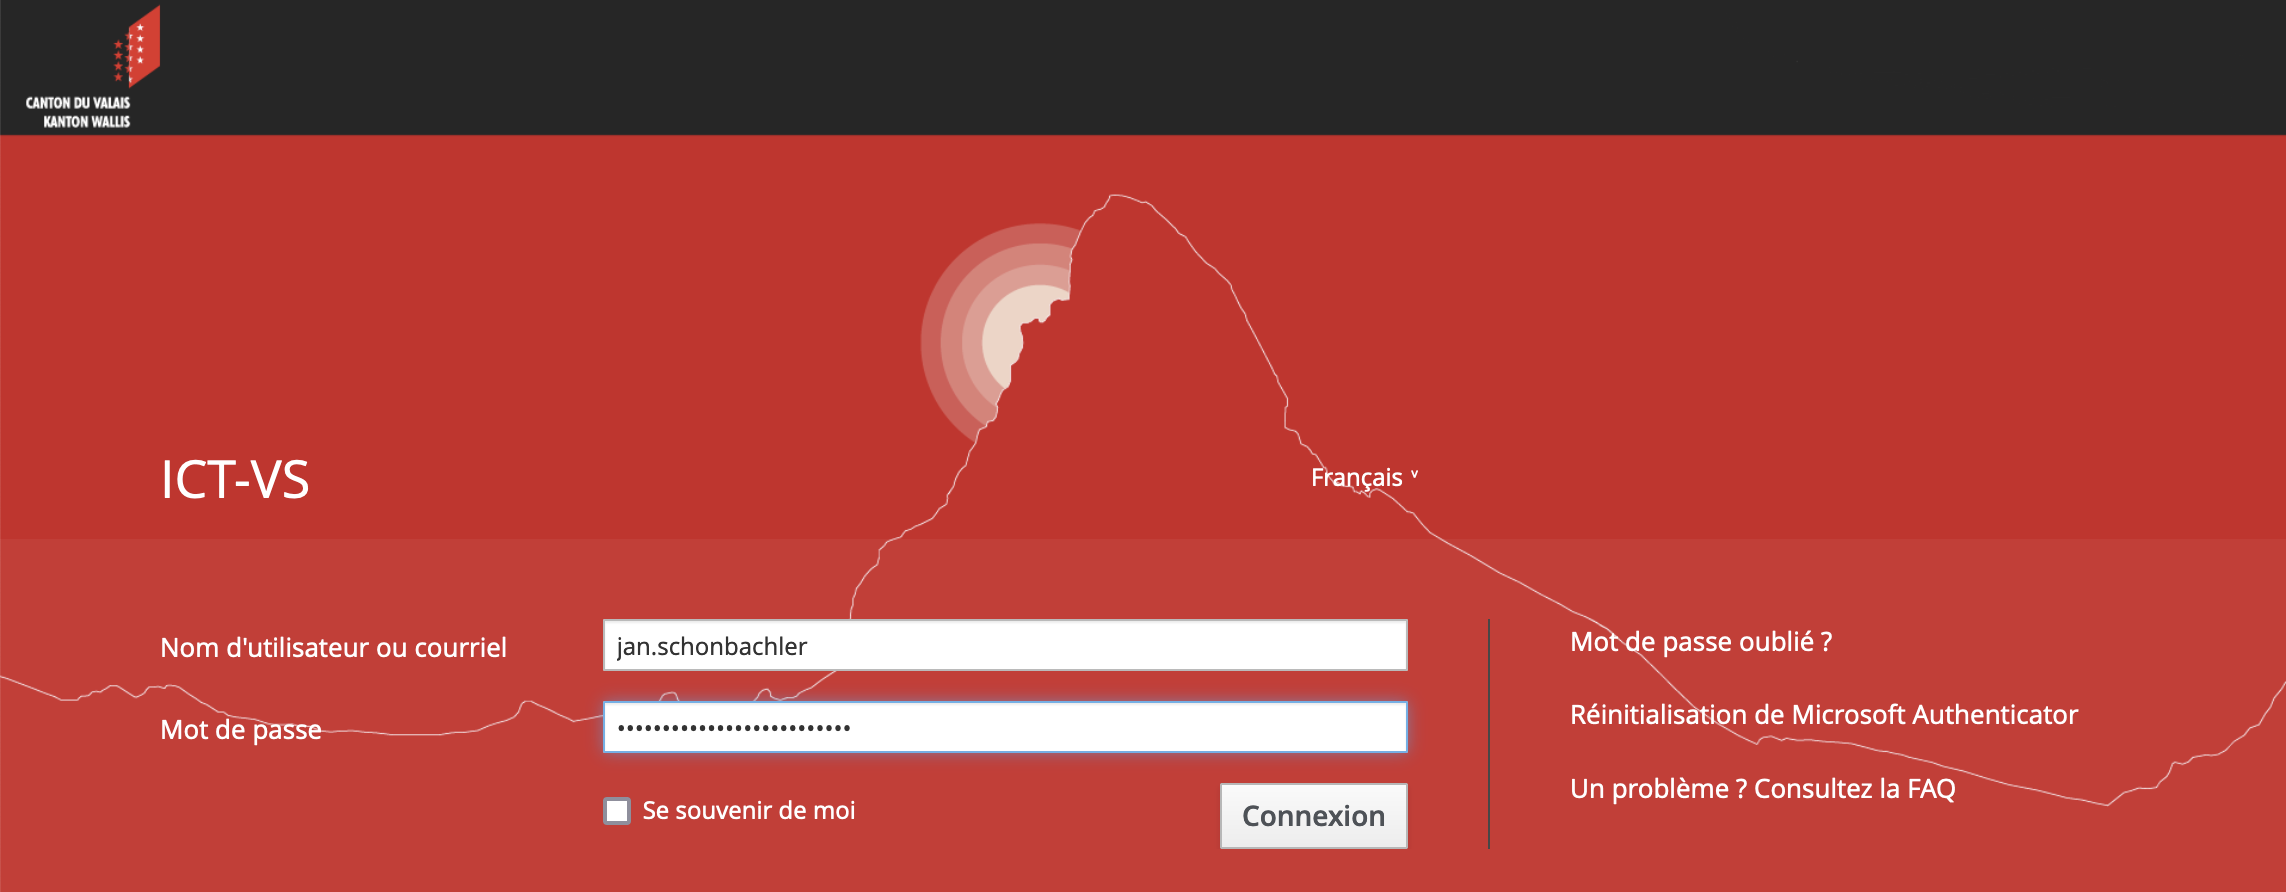
\includegraphics[width=0.8\linewidth]{images/capture_ENT_login_20210828}
		\caption{\protect \href{https://edu.vs.ch}{ENT -- Environnement numérique de travail}}
		\label{fig:accesENT}
	\end{figure}
	
	%\subsection{Plateforme d'apprentissage : Moodle}
	
	L'accès à Moodle se fait alors par la tuile Moodle marquée par une flèche dans la figure \ref{fig:accesENTversMoodle} :
	
	% TODO: \usepackage{graphicx} required
	\begin{figure}[H]
		\centering
		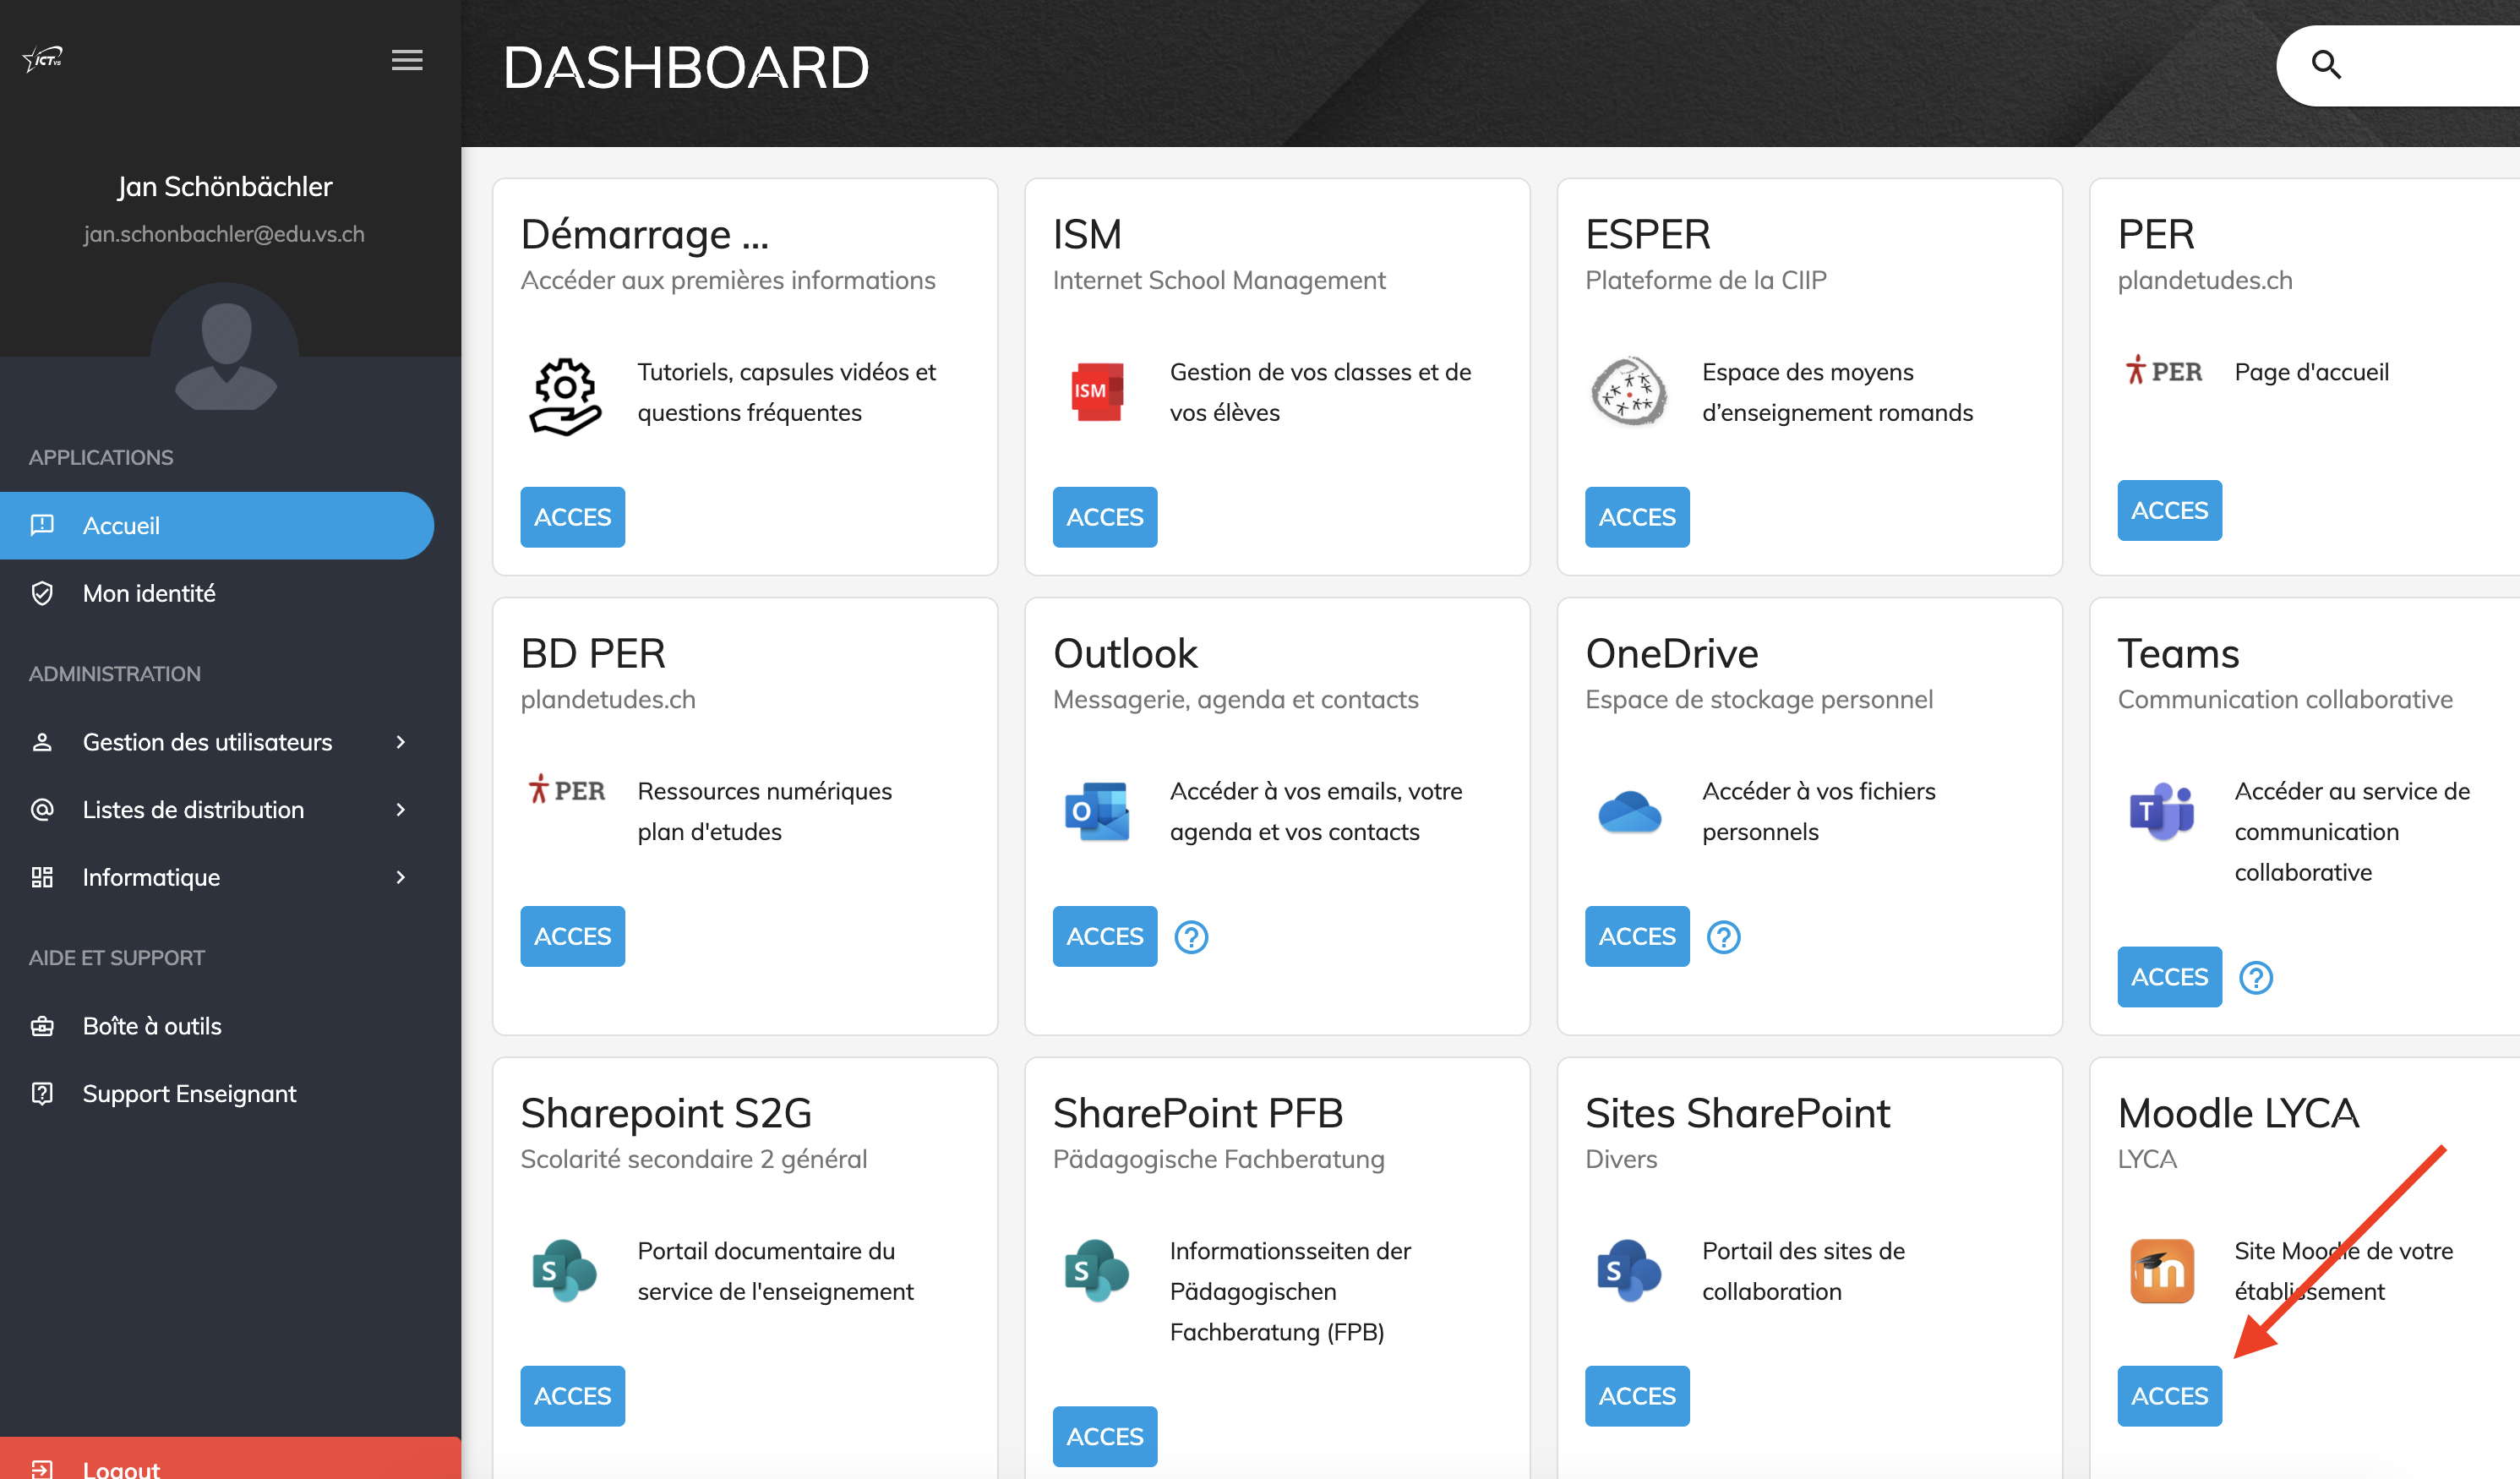
\includegraphics[width=0.8\linewidth]{images/capture_ENT_20210828}
		\caption{Accès à Moodle LYCA via l'ENT}
		\label{fig:accesENTversMoodle}
	\end{figure}
	
	
	\section{Connexion directe à \href{https://moodle.lyca.ictvs-edu.ch/}{Moodle}}
	
	Seconde possibilité : se connecter à Moodle LYCA via le lien direct\\ \href{https://moodle.lyca.ictvs-edu.ch/}{https://moodle.lyca.ictvs-edu.ch/} que vous trouvez en bas de page du site du LYCA (cf. figure \ref{fig:siteLycaLienMoodle}), ou que vous avez peut-être conservé en favori, signet ou marque-page dans votre navigateur internet.
	
	% TODO: \usepackage{graphicx} required
	\begin{figure}[H]
		\centering
		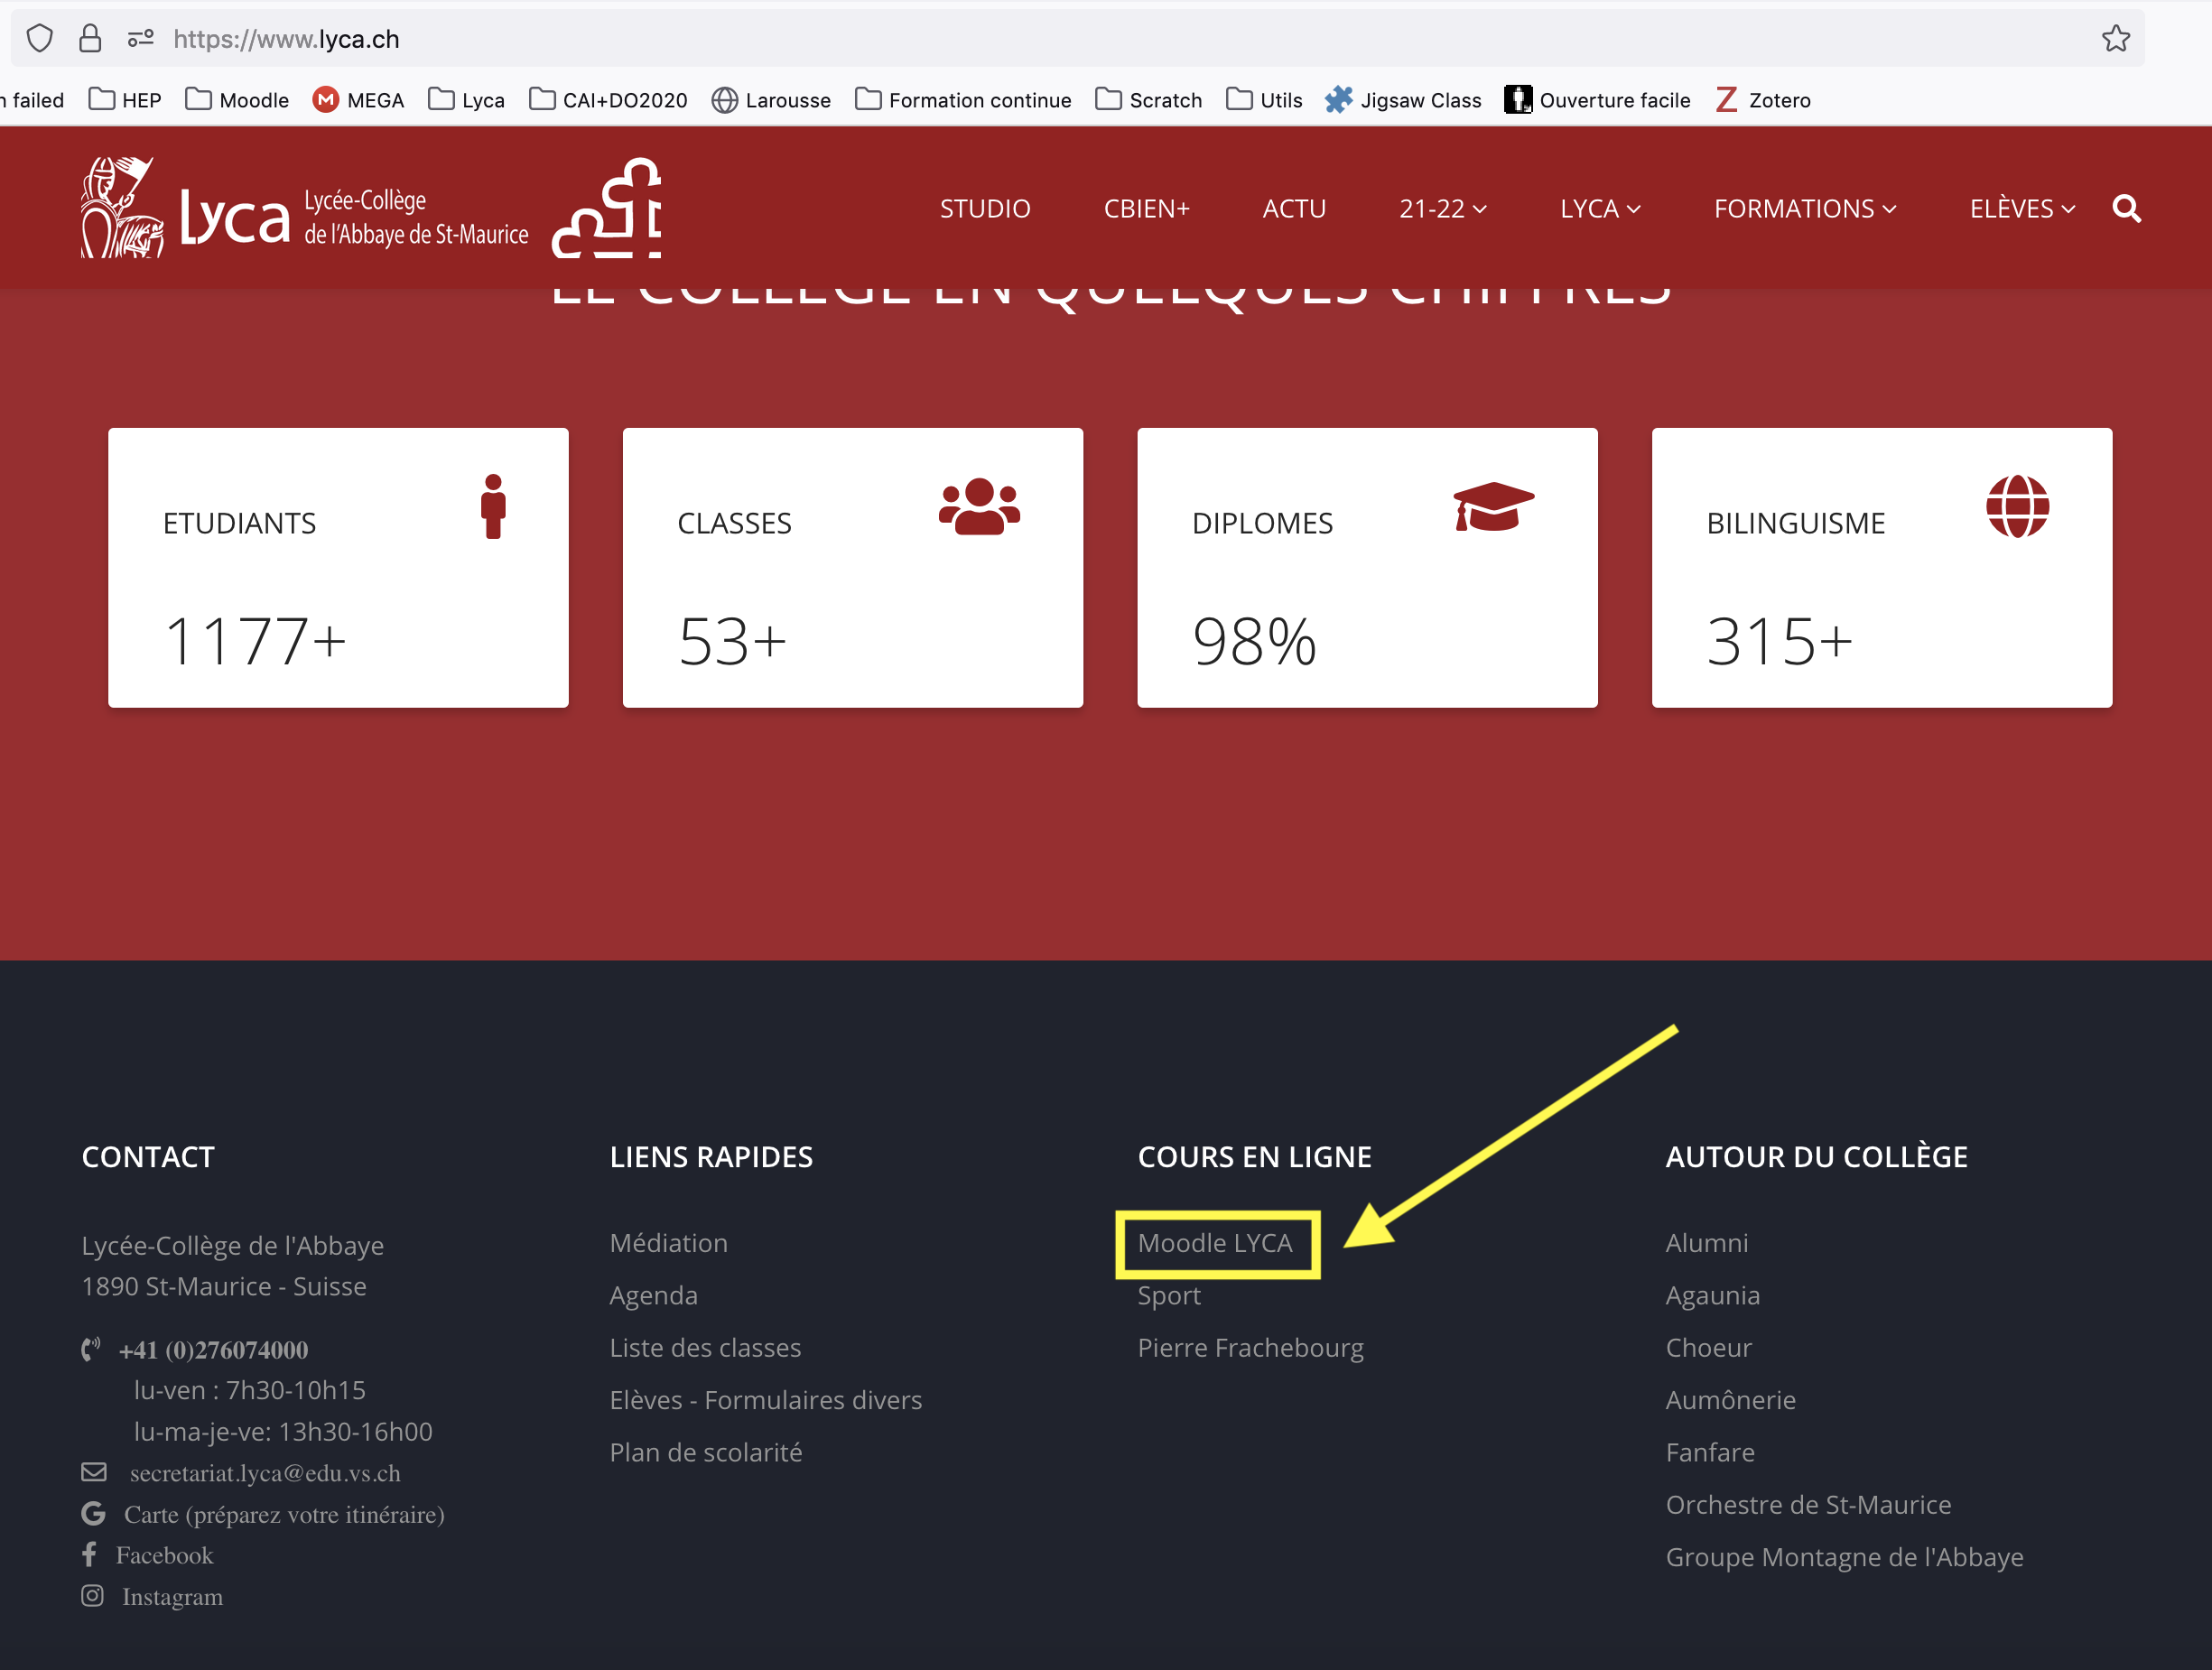
\includegraphics[width=0.8\linewidth]{images/capture_site_lyca_lien_moodle}
		\caption{Lien Moodle LYCA sur le site du Lyca}
		\label{fig:siteLycaLienMoodle}
	\end{figure}
	
	\newpage
	
	\fancyhead[LO,R]{\bfseries 2  Connexion directe à \href{https://moodle.lyca.ictvs-edu.ch/}{Moodle}}
	
	Dans ce cas, une fenêtre de connexion vous sera présentée (cf. figure \ref{fig:connexionMoodle21}), où vous devez cliquer sur le bouton "Identité unique", afin de vous connectez au moyen de votre compte "ENT".
	
	
	% TODO: \usepackage{graphicx} required
	\begin{figure}[H]
		\centering
		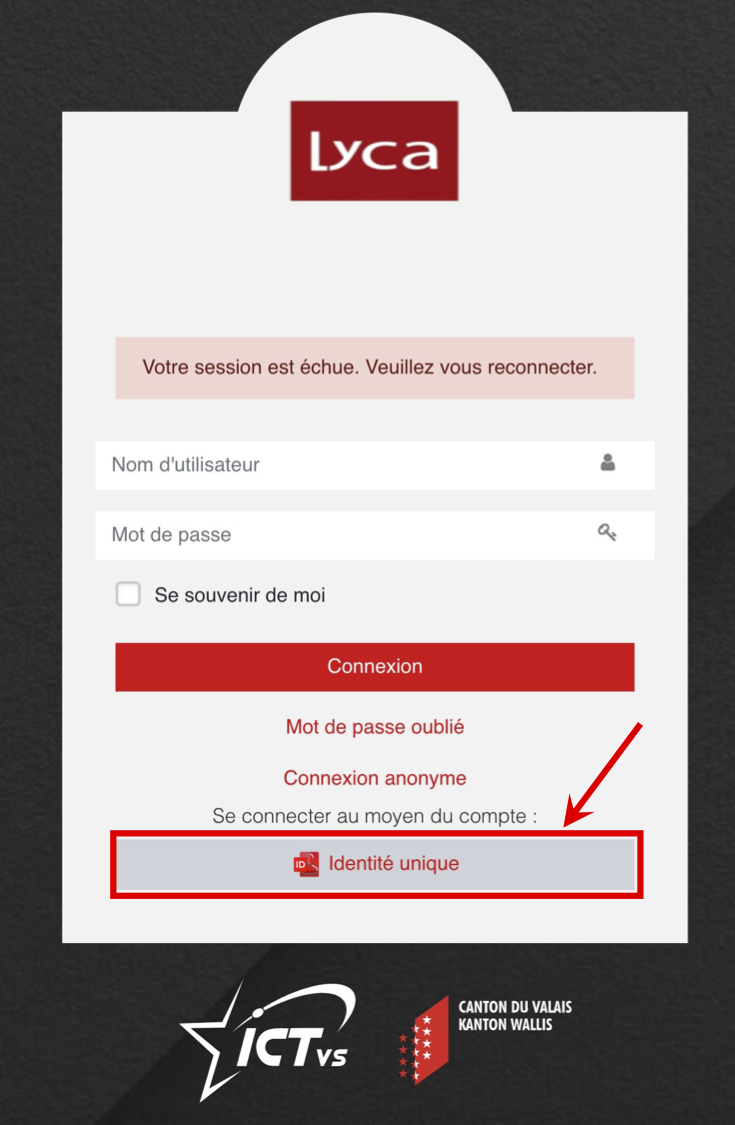
\includegraphics[width=0.48\linewidth]{images/connexion_moodle_21}
		\caption{Connexion directe à Moodle via l'identité unique}
		\label{fig:connexionMoodle21}
	\end{figure}
	
	
	\textbf{Attention :} Vous obtiendrez une erreur "La connexion a échoué, veuillez réessayer", si vous essayez de vous connecter avec votre ancien identifiant (nom d'utilisateur et mot de passe) et que vous cliquez sur le bouton rouge "Connexion" de la figure \ref{fig:connexionMoodle21}.
	
	
	Dans les deux cas, vous accéderez à votre compte Moodle, où vous retrouverez l'ensemble de vos cours, éventuellement après 24 heures, s'il s'agit de votre toute première connexion via votre identité unique.
	
	\begin{figure}[H]
		\centering
		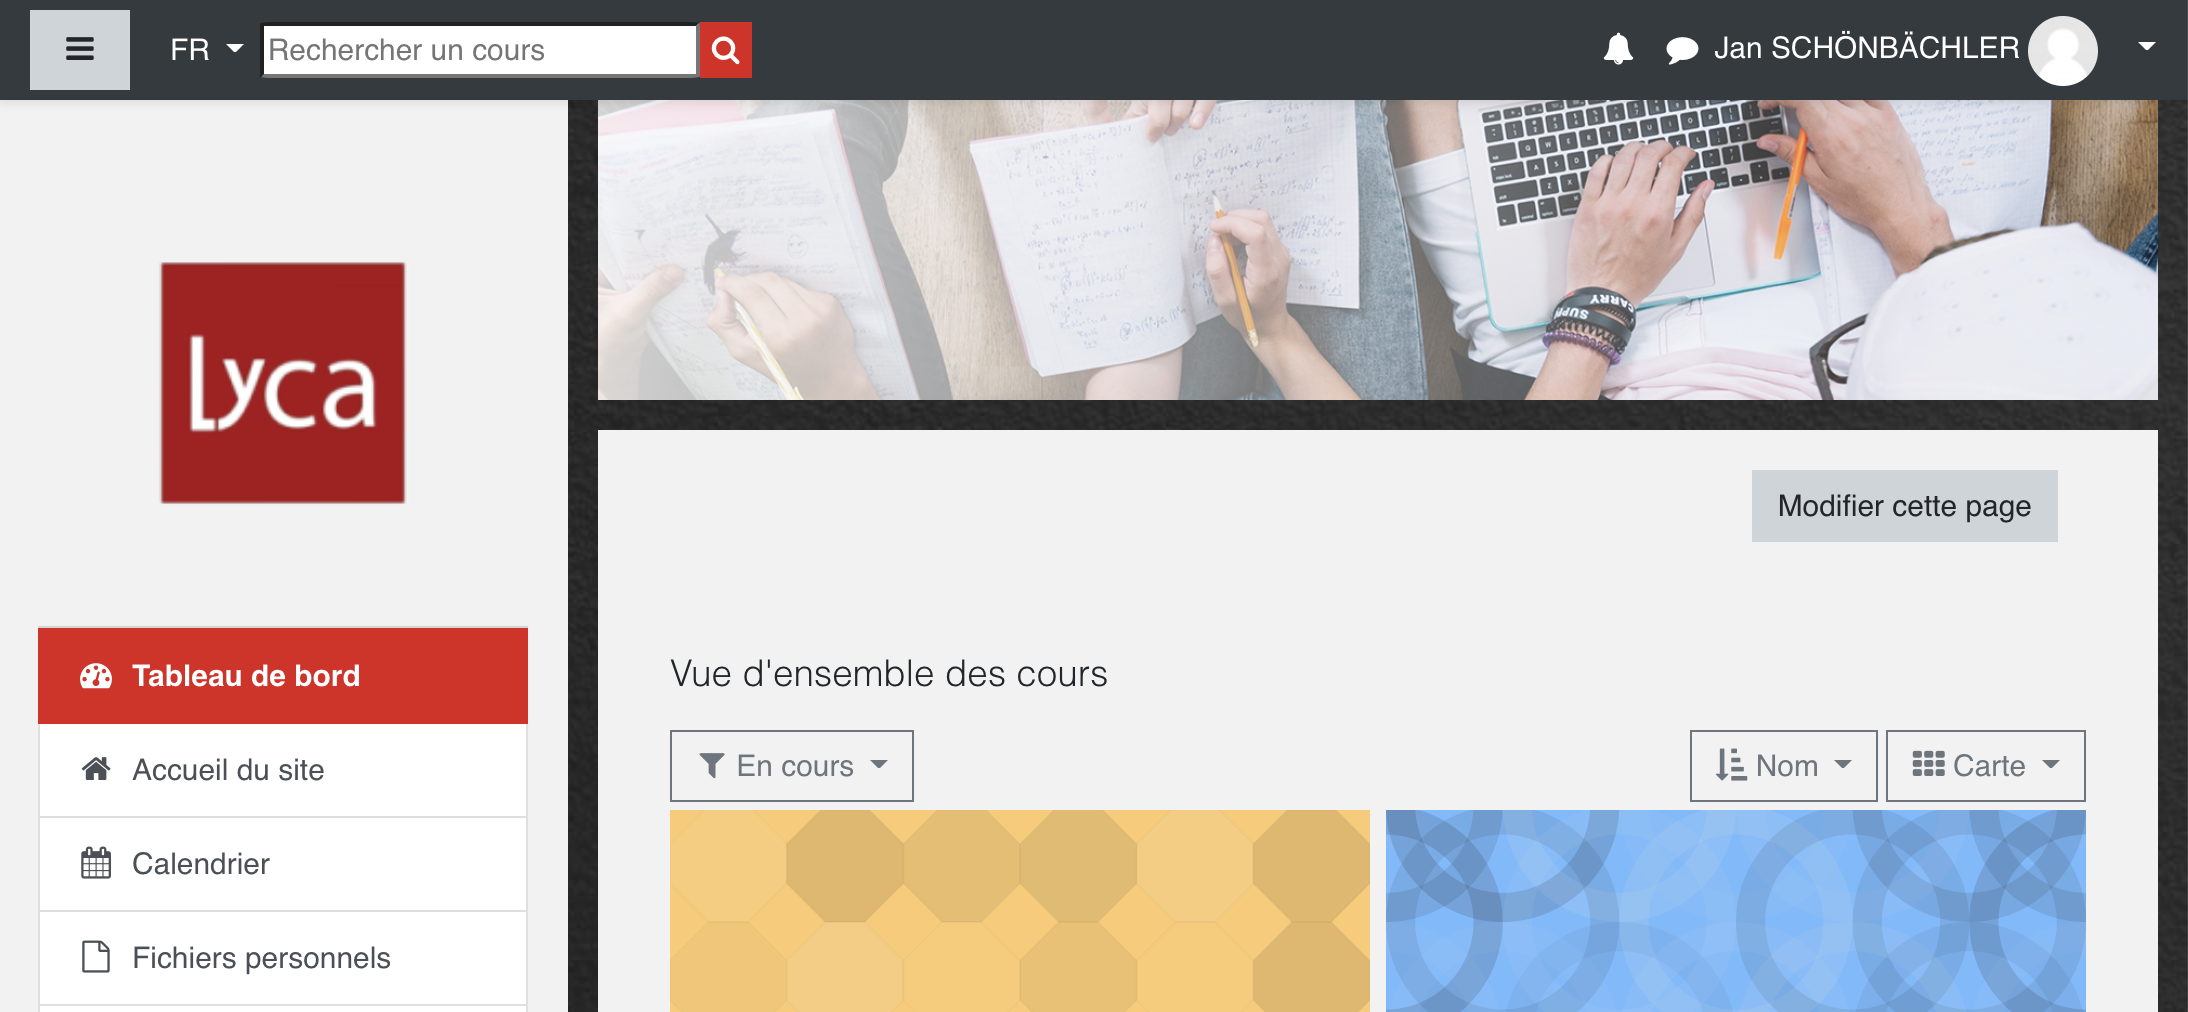
\includegraphics[width=.75\linewidth]{images/capture_moodle_lyca_2021}
		\caption{\protect{Moodle Lyca}}
		\label{fig:capturemoodlelyca}
	\end{figure}
	
\end{document}
